\documentclass[norsk]{article}
\usepackage[norsk]{babel}
\usepackage{parskip}
\usepackage[utf8]{inputenc}
\usepackage{graphicx}
\usepackage{float}
\usepackage{amsmath}

\renewcommand{\thesubsection}{\thesection.\alph{subsection}}
\author{David Kolden, davidko}

\title{UNIK 4490 - Obligatorisk oppgave 1}
\begin{document}
\maketitle
\section{}

\subsection{ }
Finner poler ved å løse \(s(1 + T_Ms) = 0\) som gir polene \(s = 0\) og \(s = -\frac{1}{T_M}\). Systemet er stabilt for alle positive verdier av \(T_M\).

\subsection{ }
Figur 1 viser blokkskjema for \(\frac{X(s)}{U(s)} = H(s) = \frac{1}{s(1 + T_Ms)}\)
\begin{figure}[!htb]
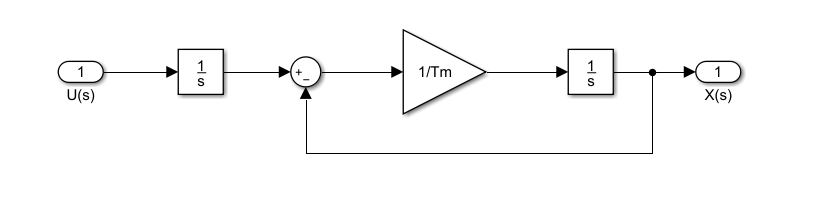
\includegraphics[height=3.5cm]{illustrations/oppg1b_illu}
\caption{Blokkskjema for \(H(s)\)}
\end{figure}

\subsection{ }
\(H(s)\) har to poler og er derfor et andreordens system.

Setter \(U(s) = K(1 + T_Ds)E(s)\), \(E(s) = R(s) - X(s)\), \(U(s) = K(1 + T_Ds)(R(s) - X(s))\) sammen med \(H(s)\):
\[X(s) = H(s)U(s) = H(s)K(1+T_Ds)(R(s) - X(s))\] 
\[X(s) = H(s)K(1+T_Ds)R(s) - H(s)K(1+T_Ds)X(s)\]
\[X(s)(1 + H(s)K(1+T_Ds)) = H(s)K(1+T_Ds)R(s)\]
\[\frac{X(s)}{R(s)} = H_C(s) = \frac{H(s)K(1+T_Ds)}{1+H(s)K(1+T_Ds)}\]
\[H_C(s) = \frac{K(1+T_Ds)}{\frac{1}{H(s)} + K(1+T_Ds)}\]

Setter inn for \(H(s)\):
\[H_C(s) = \frac{K(1+T_Ds)}{s(1+T_Ms)+ K(1+T_Ds)}\]
\[H_C(s) = \frac{K(1+T_Ds)}{s^2T_M + s + KT_Ds + K}\]
\[H_C(s) = \frac{(1+T_Ds)}{s^2\frac{T_M}{K} + s(\frac{1}{K}+T_D) + 1}\]

Ser at systemet med kontroller fortsatt er et andreordens system.
\subsection{ }
Figur to viser blokkskjema for systemet med kontroller (\(H_C(s)\))
\begin{figure}[!htb]
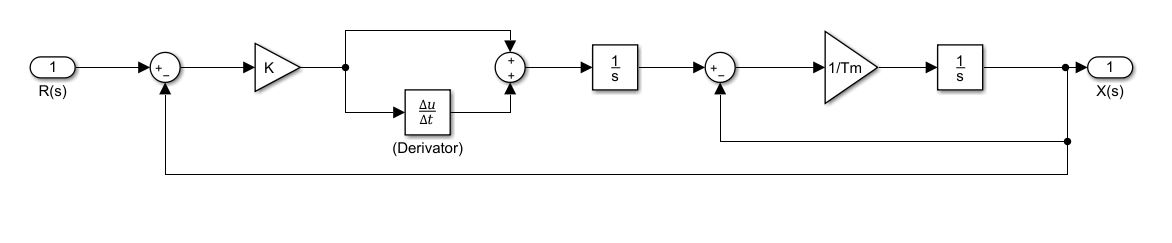
\includegraphics[height=2.9cm]{illustrations/oppg1d_illu}
\caption{Blokkskjema for \(H_C(s)\)}
\end{figure}

\subsection{ }
\(H_C(s)\) har ett nullpunkt og to poler. Nullpunktet finnes ved å sette telleren i \(H_C(s)\) til null, mens man finner polene ved å sette nevneren til null. Polene kan dermed finnes med uttrykket
\[s = \frac{-(\frac{1}{K} + T_D) \pm \sqrt{(\frac{1}{K} + T_D)^2 - 4\frac{T_M}{K}}}{2\frac{T_M}{K}}\]

mens nullpunktene finnes med uttrykket
\[s = -\frac{1}{T_D}\]

Ved å sette inn for \(T_M = 2\) og \(T_D = 1\) får vi til slutt et nullpunkt i \(s = -1\) og to poler i
\[s = \frac{-(\frac{1}{K} + 1) \pm \sqrt{(\frac{1}{K} + 1)^2 - 4\frac{2}{K}}}{2\frac{2}{K}} = \frac{-(1+K)}{4}\pm\frac{\sqrt{(1+K)^2-8K}}{4}\]
Realdelen til polene vil være negative for alle \(K > 0\). Systemet er derfor asymptotisk stabilt for alle \(K>0\). Polene vil ha en imaginærdel for \(5.83 > K > 0.17\). Da er systemet underdempet ettersom \(0 < \zeta < 1\), og vil derfor overskyte og svinge seg inn mot settpunkt. Dempningsfaktoren \(\zeta\) gis som \(\frac{1+KT_D}{2\sqrt{TMK}} = \frac{1+K}{2\sqrt{2K}}\), og den udempede resonansfrekvensen gis av \(\sqrt{\frac{K}{T_M}} = \sqrt{\frac{K}{2}}\).

\begin{figure}[H]
\hspace{-2cm}
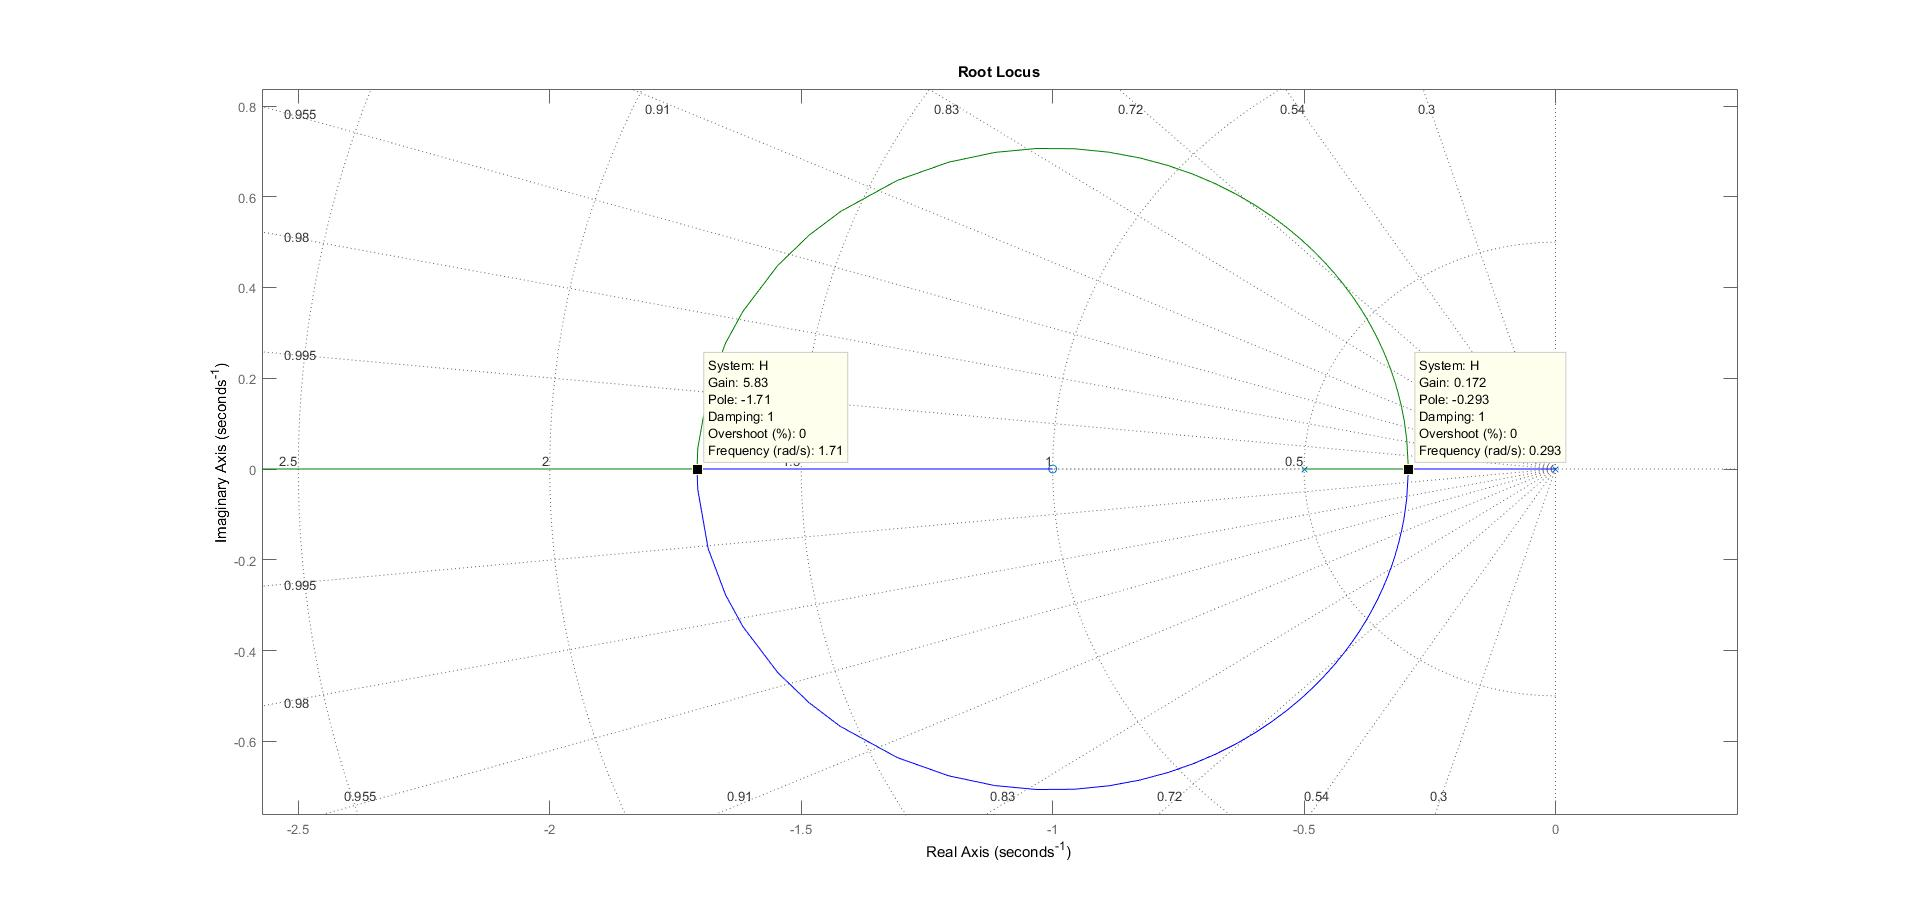
\includegraphics[height=8.5cm]{illustrations/oppg1e_illu}
\caption{Locusplot av \(H_C\)}
\end{figure}

\section{}
Et system kan verifiseres som stabilt for en kandidatfunksjon \(V(x,y)\) hvis
\begin{itemize}
\item \(V(x, y) > 0 \qquad \forall x \neq 0, y \neq 0\)
\item \(V(x,y) = 0 \qquad x = y = 0\)
\item \(V(x,y) \rightarrow \infty \qquad x \rightarrow \infty, y \rightarrow \infty\)
\item \(\dot{V}(x,y) < 0 \)
\end{itemize}
Med en kandidatfunksjon \[V(x,y) = x^2 +  y^2\] ser vi at kravene fra første, andre og tredje punkt er godkjente ettersom begge uttrykkene er kvadratiske.

Med systemet \[\dot{x} = -y-x^3\] \[\dot{y} = x - y^3\] kan systemet verifiseres ved å finne \(\dot{V}(x, y)\).

\[\dot{V}(x,y) = 2x\dot{x} + 2y\dot{y}\]
\[\dot{V}(x,y) = 2x(-y-x^3) + 2y(x-y^3)\]
\[\dot{V}(x,y)=-2xy-2x^4 + 2xy-2y^4\]
\[\dot{V}(x,y) = -x^4-y^4\]

Vi ser at \(\dot{V}(x,y)\) er godkjent i forhold til det siste kravet ettersom \(x^4\) og \(y^4\) ikke kan bli negative.



\section{}
\subsection{ }
En PD-kontroller med gravitasjonskompensasjon består av et proporsjonalledd, et derivatledd og et ledd som kompenserer for gravitasjonskreftene på manipulatoren. Proporsjonalleddet forsterker avviket mellom ønsket leddposisjon \(q_d\) og faktisk leddposisjon \(q\). Derivatleddet forsterker leddhastighetene til manipulatoren og trekker det fra pådraget. Gravitasjonskreftene forandrer seg som funksjon av leddposisjonene. Det fulle uttrykket for kontrolleren er 
\[u = K_P(q_d - q) - K_D\dot{q} + g(q)\]
hvor \begin{itemize}

\item \(K_P = \begin{bmatrix}
k_{p1} & 0 \\
0 & k_{p2}
\end{bmatrix}\)
\item \(K_D = \begin{bmatrix}
k_{d1} & 0 \\
0 & k_{d2}
\end{bmatrix}\)
\item \(q_d = \begin{bmatrix}
\vartheta_{d1} \\ \vartheta_{d2}
\end{bmatrix}\)
\item \(q = \begin{bmatrix}
\vartheta_1 \\ \vartheta_2
\end{bmatrix}\)
\item \(\dot{q} = \begin{bmatrix}
\dot{\vartheta_1} \\ \dot{\vartheta_2}
\end{bmatrix}\)
\item \(g(q) = \begin{bmatrix}
(m_{l1}l_1+m_{m2}a_1+m_{l2}a_1)gcos(\vartheta_1) + m_{l2}l_2gcos(\vartheta_1 + \vartheta_2) \\ m_{l2}l_2gcos(\vartheta_1 + \vartheta_2)
\end{bmatrix}\)

hvor
\begin{itemize}
\item \(m_{l1} = 50\) kg og er massen til \(link_1\).
\item \(m_{l2} = 50\) kg og er massen til \(link_2\).
\item \(m_{m2} = 5\) kg og er massen til \(motor_2\).
\item \(l_1 = 0.5\) m og er avstanden fra starten av \(link_1\) til \(link_1\)s
tyngdepunkt.
\item \(l_2 = 0.5\) m og er avstanden fra starten av \(link_2\) til \(link_2\)s tyngdepunkt.
\item \(a_1 = 1\) m og er lengden til \(link_1\).
\item \(a_2 = 1\) m og er lengden til \(link_2\).
\item \(\vartheta_1\) er vinkelen til \(ledd_1\).
\item \(\vartheta_2\) er vinkelen til \(ledd_2\).
\item \(g = 9.81\) \(m/s^2\).
\end{itemize}
\end{itemize}
Dette gir følgende uttrykk for pådraget \(u\):
\[
u = 
\begin{bmatrix}
k_{p1} & 0 \\
0 & k_{p2}
\end{bmatrix}
\begin{bmatrix}
\vartheta_{d1} - \vartheta_1\\ \vartheta_{d2} - \vartheta_2
\end{bmatrix}
-
\begin{bmatrix}
k_{d1} & 0 \\
0 & k_{d2}
\end{bmatrix}
\begin{bmatrix}
\dot{\vartheta_1} \\ \dot{\vartheta_2}
\end{bmatrix}
+
\begin{bmatrix}
(m_{l1}l_1+m_{m2}a_1+m_{l2}a_1)gcos(\vartheta_1) + m_{l2}l_2gcos(\vartheta_1 + \vartheta_2) \\ m_{l2}l_2gcos(\vartheta_1 + \vartheta_2)
\end{bmatrix}\
\] 
\subsection{ }
Blokkskjema for kontroller og manipulator gis i figur 4 og figur 5.
\begin{figure}[H]
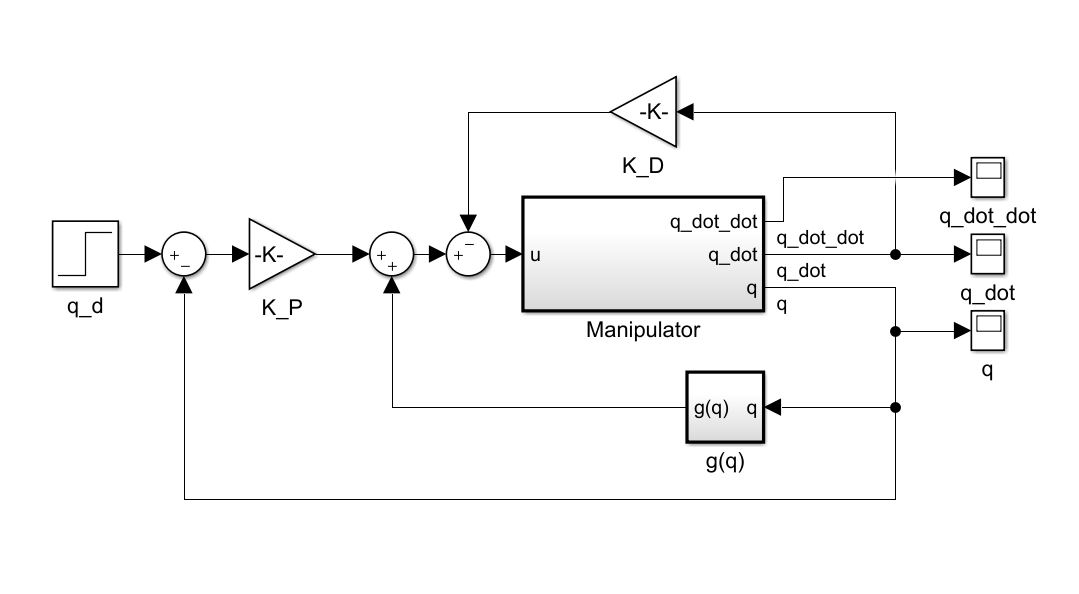
\includegraphics[height=6cm]{illustrations/oppg3b_illu1}
\caption{Blokkskjema for PD-kontroller med gravitasjonskompensasjon}
\end{figure}

\begin{figure}[H]
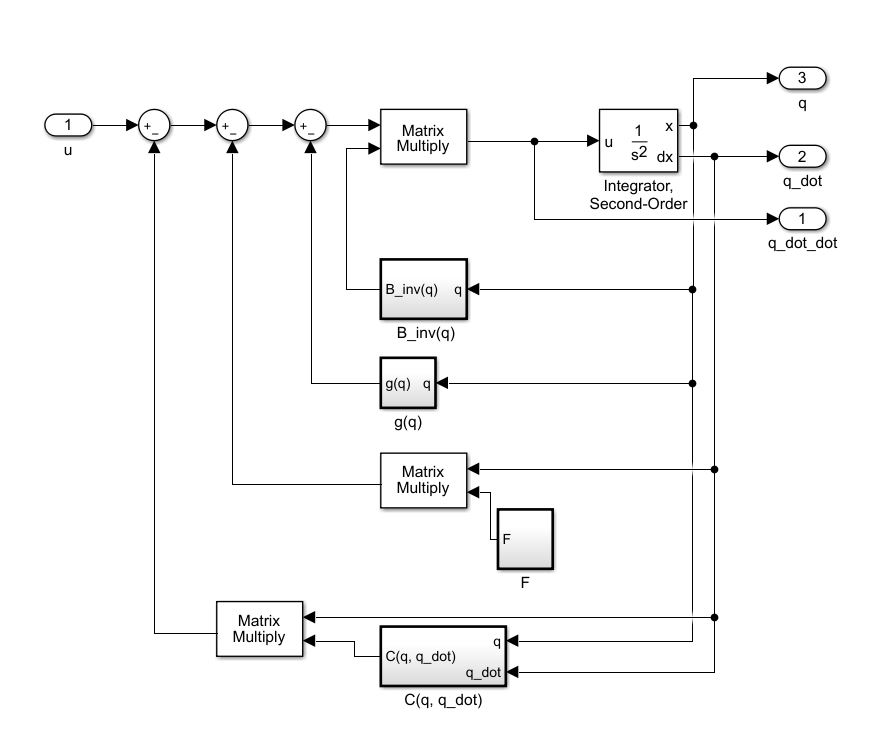
\includegraphics[height=10cm]{illustrations/oppg3b_illu2}
\caption{Blokkskjema for maniplator. Matrisen B er funksjon av \(q\), C er funksjon av \(q\) og \(\dot{q}\), mens vektoren g er funksjon av \(q\).}
\end{figure}

\subsection{ }
\(K_P\) og \(K_D\) ble satt til \(2400I\) og \(1300I\). Figur 6 viser sprangrespons for \(\vartheta_1\), \(ledd_1\), figur 7 viser sprangrespons for \(\vartheta_2\), \(ledd_2\).

\begin{figure}[H]
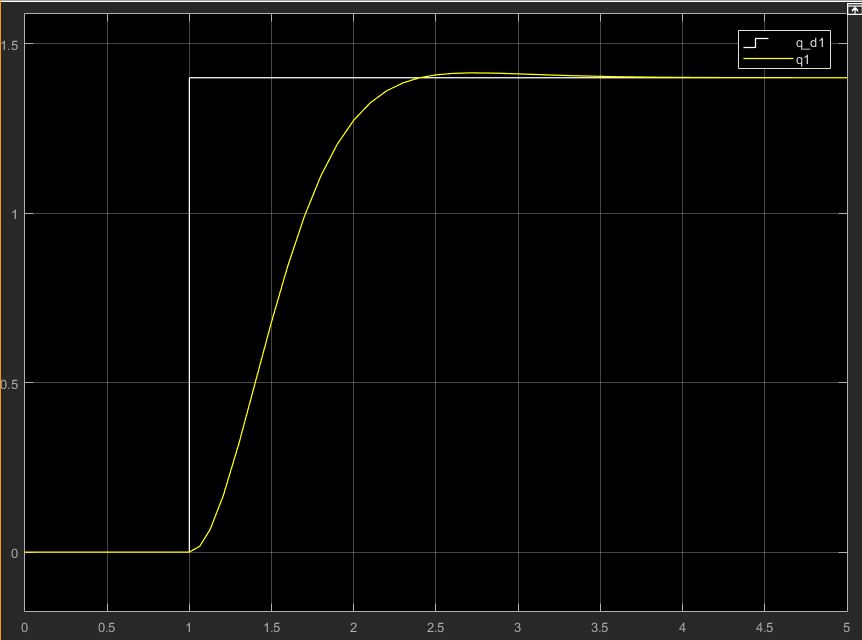
\includegraphics[height=7.2cm]{illustrations/oppg3c_illu1}
\caption{Plot av \(\vartheta_1\)s (gult) respons på spranget i \(\vartheta_{d1}\) (hvitt).}
\end{figure}

\begin{figure}[H]
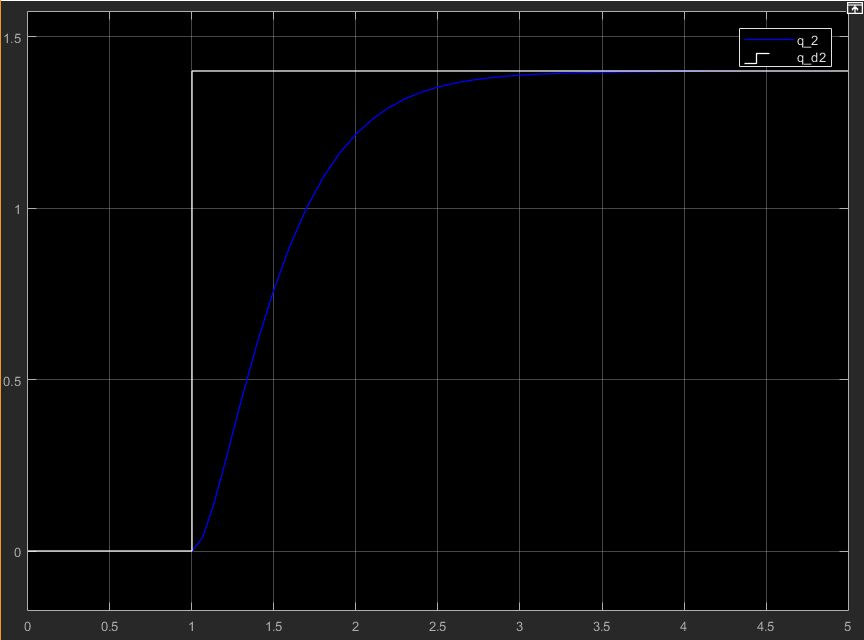
\includegraphics[height=7.2cm]{illustrations/oppg3c_illu2}
\caption{Plot av \(\vartheta_2\)s (blått) respons på spranget i \(\vartheta_{d2}\) (hvitt).}
\end{figure}
\subsection{ }
Med invers dynamikkontroll vil vi ha et pådrag \(u\) slik at
\[u = B(q)y + n(q, \dot{q})\]
hvor \(n(q, \dot{q}) = C(q, \dot{q})\dot{q}+F_v\dot{q} + g(q)\). Målet er å ende opp med \(y = \ddot{q}\).

Representerer \(y\) med
\[y = -K_Pq -K_D\dot{q} + r\]
og setter
\[r = \ddot{q}_d + K_D\dot{q}_d + K_Pq_d\]
Setter representasjonen av \(r\) inn i \(y\) og får
\[y = \ddot{q_d} + K_D\dot{\tilde{q}} + K_P\tilde{q}\]
hvor \(\tilde{q} = q_d - q\).

Setter y inn i uttrykket for \(u\) og får
\[u = B(q)(\ddot{q_d} + K_D\dot{\tilde{q}} + K_P\tilde{q}) + C(q, \dot{q})\dot{q}+F_v\dot{q} + g(q)\]
\subsection{ }
Blokkskjema for invers dynamikkontroller gis i figur 8.
\begin{figure}[H]
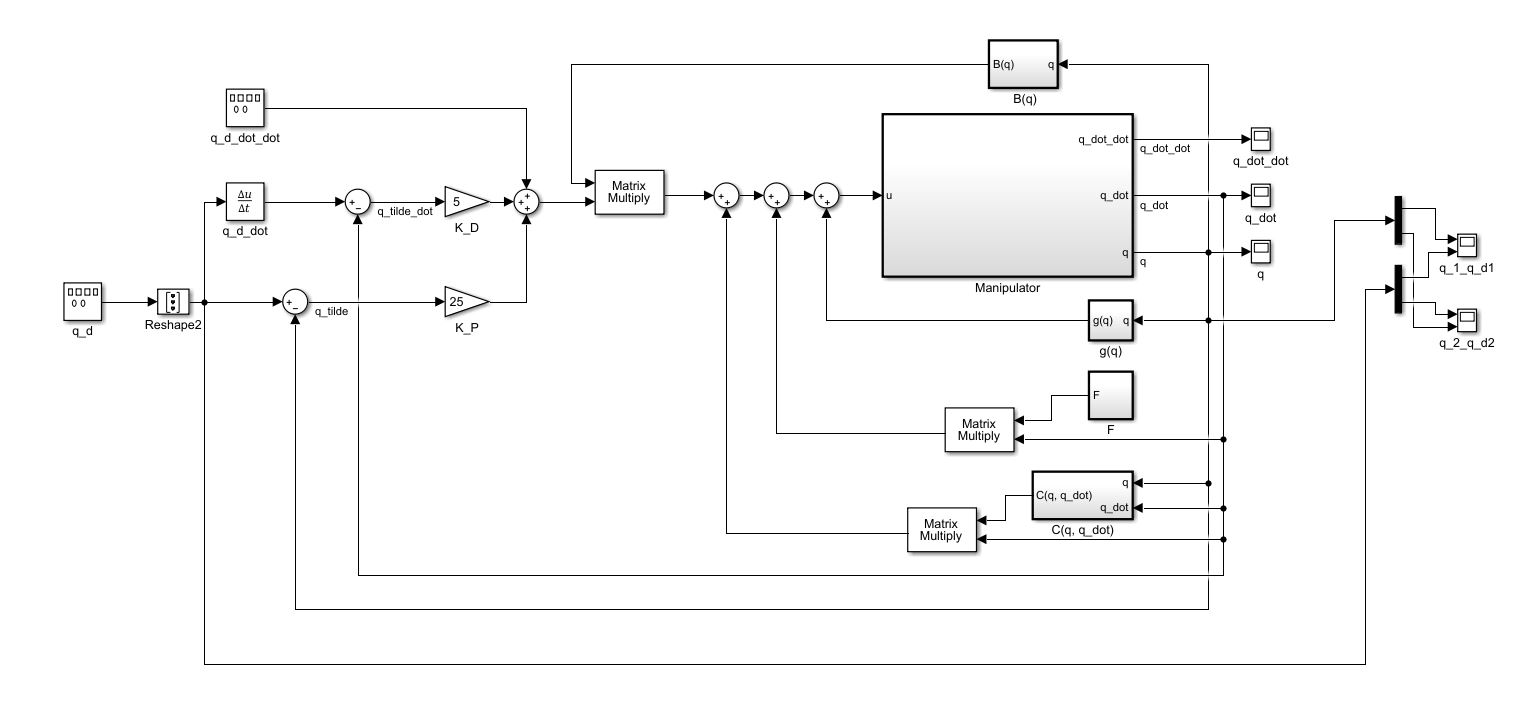
\includegraphics[height=7.5cm]{illustrations/oppg3e_illu1}
\caption{Blokkskjema for invers dynamikkontroller. \(q_d\) ble generert som et sinus-signal, mens \(\dot{q}_d\) ble generert som den deriverte av sinus-signalet. \(\ddot{q}_d\) ble generert som eget signal på samme måte som \(q_d\).}
\end{figure}
\subsection{ }
\begin{itemize}
\item For \(f = 0.5\) Hz:
\begin{figure}[H]
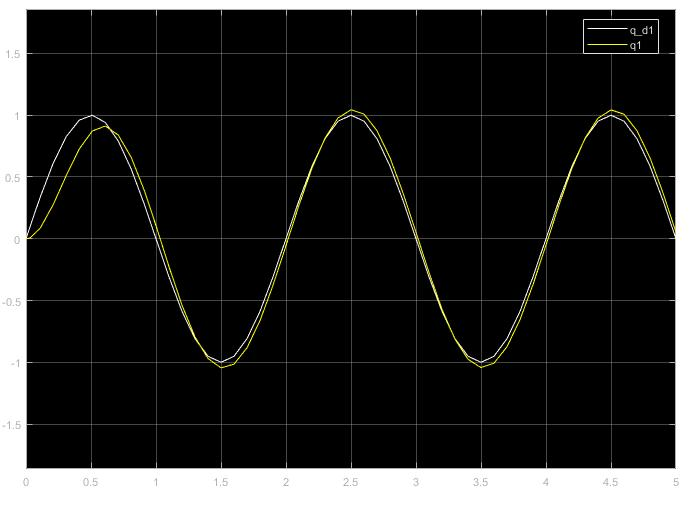
\includegraphics[height=7cm]{illustrations/oppg3f_illu1}
\caption{\(q_1\) følger pådraget relativt godt. Det er et lite avvik i oppstarten på ca 0.1.}
\end{figure}
\begin{figure}[H]
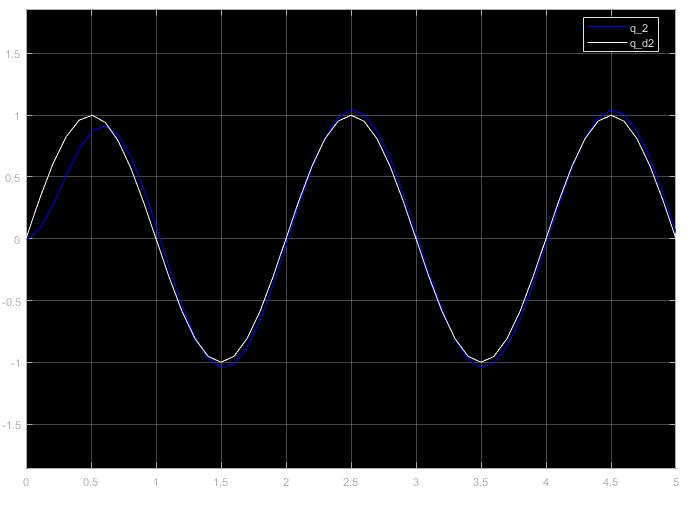
\includegraphics[height=7cm]{illustrations/oppg3f_illu2}
\caption{\(q_2\) følger pådraget på samme måte som \(q_1\).}
\end{figure}
\item For \(f = 1.0\) Hz:

\begin{figure}[H]
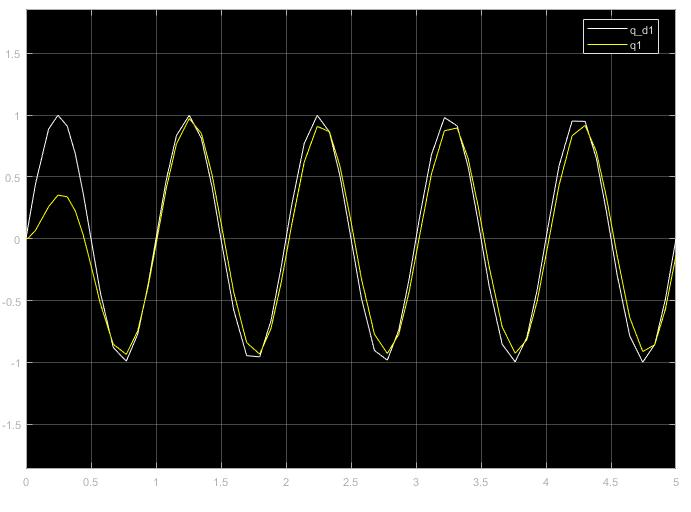
\includegraphics[height=7cm]{illustrations/oppg3f_illu3}
\caption{Ved 1,0 Hz ses det et tydeligere avvik i oppstarten. Avviket i amplituden er på ca 0.6.}
\end{figure}
\begin{figure}[H]
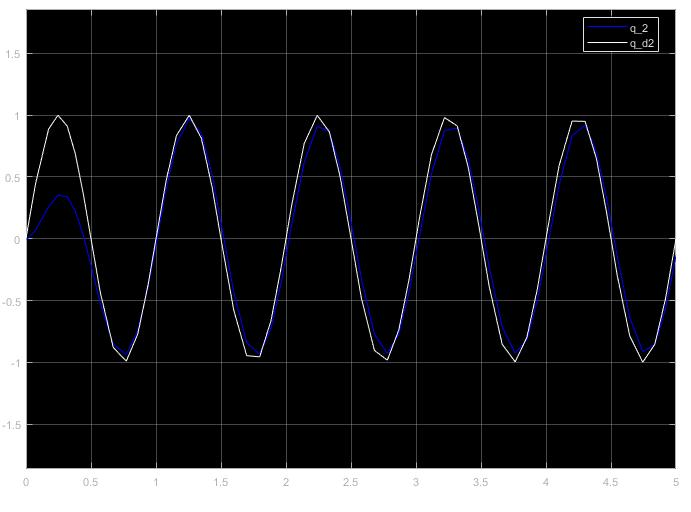
\includegraphics[height=7cm]{illustrations/oppg3f_illu4}
\caption{\(q_2\) følger pådraget på samme måte som \(q_1\).}
\end{figure}

\newpage
\item For \(f = 2.0\) Hz:

\begin{figure}[H]
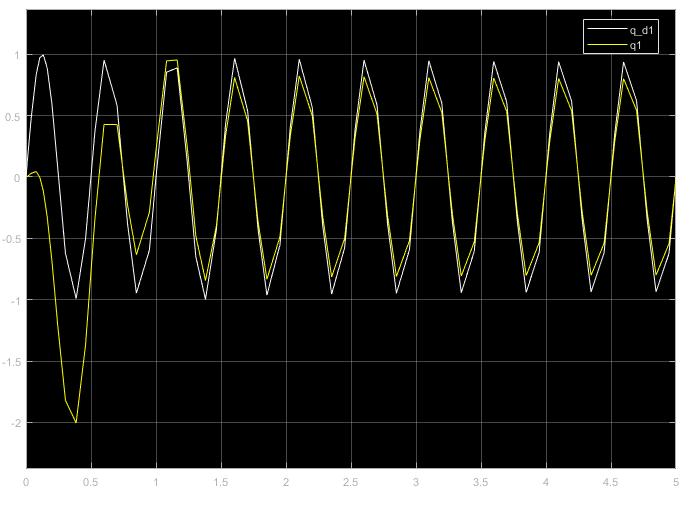
\includegraphics[height=7cm]{illustrations/oppg3f_illu5}
\caption{Systemet får større og større avvik i oppstarten av systemet. Avviket er på ca 1.}
\end{figure}
\begin{figure}[H]
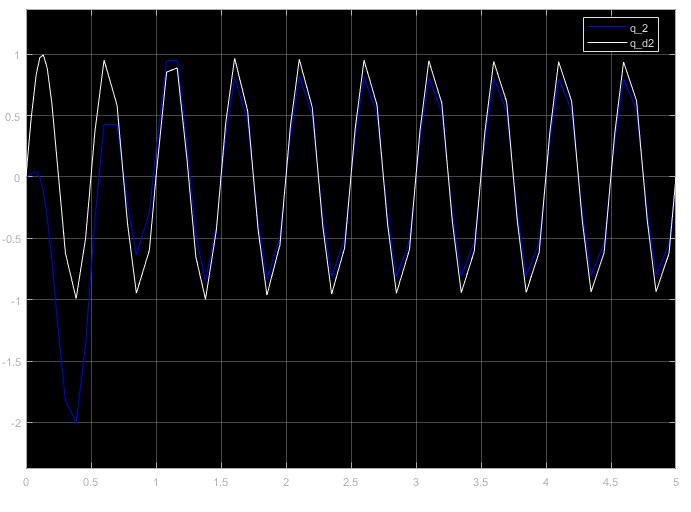
\includegraphics[height=7cm]{illustrations/oppg3f_illu6}
\caption{\(q_2\) følger pådraget på samme måte som \(q_1\).}
\end{figure}
\end{itemize}
Det ses at avviket øker med frekvensen i pådraget. Dempningen \(\zeta\) og den udempede resonansfrekvensen \(\omega_n\) gis av \(K_P\) og \(K_D\):

\[K_P = \begin{bmatrix}
\omega_{n1}^2 & 0 \\ 0 & \omega_{n2}
\end{bmatrix} 
= 
\begin{bmatrix}
25 & 0 \\ 0 & 25 
\end{bmatrix}
=
\begin{bmatrix}
5^2 & 0 \\ 0 & 5^2
\end{bmatrix}\]

\[K_D = \begin{bmatrix}
2\zeta_1\omega_{n1} & 0 \\ 0 & 2\zeta_1\omega_{n2}
\end{bmatrix} 
= 
\begin{bmatrix}
5 & 0 \\ 0 & 5 
\end{bmatrix}
\]
Dette gir \(\zeta_1 = \zeta_2 = 0.5\). Et system er underdempet når \(0 < \zeta < 1\). Derfor er dette systemet underdempet. 
\subsection{ }
Et kritisk dempet system har \(\zeta = 1\). Da må \(K_D\) justeres:
\[K_D = \begin{bmatrix}
2\zeta_1\omega_{n1} & 0 \\ 0 & 2\zeta_1\omega_{n2}
\end{bmatrix} 
= 
\begin{bmatrix}
2 \cdot 1 \cdot 5 & 0 \\ 0 & 2 \cdot 1 \cdot 5 
\end{bmatrix}
= 
\begin{bmatrix}
10 & 0 \\ 0 & 10 
\end{bmatrix}
\]
Figur 15 og figur 16 viser plot av simulering med nye verdier for \(K_D\).

\begin{figure}[H]
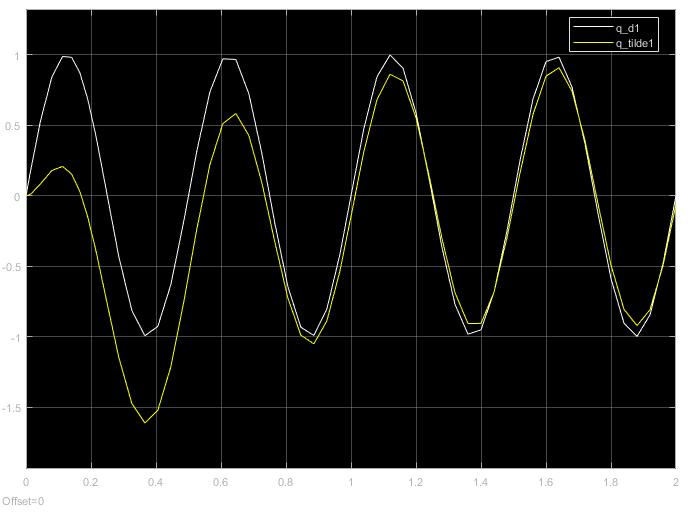
\includegraphics[height=7cm]{illustrations/oppg3g_illu1}
\caption{Responsen til \(q_1\). Responsen er forbedret.}
\end{figure}

\begin{figure}[H]
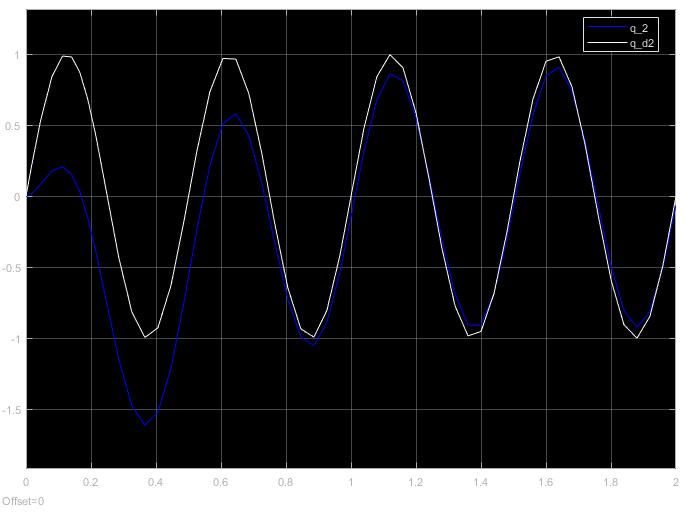
\includegraphics[height=7cm]{illustrations/oppg3g_illu2}
\caption{Viser samme resultat som for \(q_1\).}
\end{figure}

\subsection{ }
Har at \(\tilde{B} = \hat{B} - B\) og \(\tilde{n} = \hat{n} - n\). Som sagt i oppgave \(3d\), så er målet med kontrolleren å få \(\ddot{q} = y\), men siden vi har unøyaktigheter i den matematiske modellen av robotarmen i kontrolleren, så får vi en feil \(\eta\) som legges til, og vi ender opp med \(\ddot{q} = y + \eta\). I vårt eksempel er \(\hat{B} = 0.90B\) og \(\hat{n} = 0.95n\). Dette gjør at signalet aldri når opp til settpunkt, og differansen blir større jo mindre \(\hat{B}\) er i forhold til \(B\).
\begin{figure}[H]
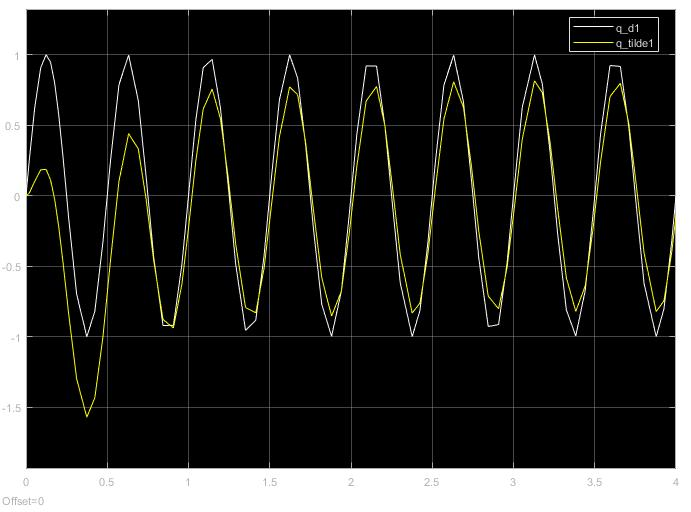
\includegraphics[height=7cm]{illustrations/oppg3h_illu1}
\caption{.}
\end{figure}

\begin{figure}[H]
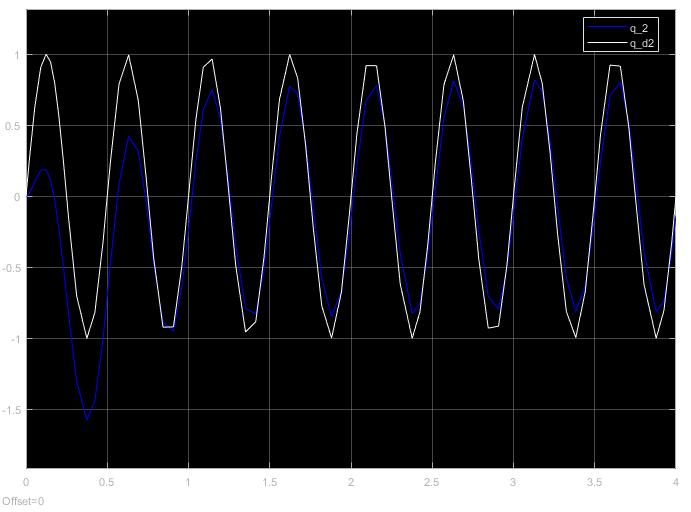
\includegraphics[height=7cm]{illustrations/oppg3h_illu2}
\caption{Viser samme resultat som for \(q_1\).}
\end{figure}
\end{document}